\documentclass{article}
\usepackage[utf8]{inputenc}
\usepackage{amsmath, amssymb, mathtools, graphicx}

\graphicspath{{Images/}}

\setlength{\oddsidemargin}{0in}
\setlength{\textwidth}{6.5in}
\setlength{\topmargin}{-.55in}
\setlength{\textheight}{9in}
\pagestyle{empty}

\title{Scientific Computation Final}
\author{Michael Nameika}
\date{December 2022}

\begin{document}

\maketitle

\section*{Exercise 1.}
Let $h > 0$.
\begin{itemize}
    \item[(a)] Use Taylor series expansion to show the following one-sided finite difference scheme is second order accurate, that is
    \[u'(x) = \frac{1}{2h}[3u(x) - 4u(x - h) + u(x - 2h)] + \mathcal{O}(h^2)\]

    Let us begin by Taylor expanding each of the terms above:
    \begin{align*}
        u(x) &= u(x) \\
        u(x-h) &= u(x) - hu'(x) + \frac{h^2}{2}u''(x) - \frac{h^3}{3!}u'''(x) + \mathcal{O}(h^4) \\
        u(x-2h) &= u(x) - 2hu'(x) + 2h^2u''(x) - \frac{8h^3}{3!}u'''(x) + \mathcal{O}(h^4) \\
    \end{align*}
    Then we have
    \begin{align*}
        &3u(x) - 4u(x-h) + u(x-2h) = \\ 
        &3u(x) -4u(x) + 4hu'(x) - 2h^2u''(x) - \frac{2}{3}u'''(x) + u(x) - 2hu'(x) + 2h^2u''(x) - \frac{8h^3}{3!}u'''(x) + \mathcal{O}(h^4) \\
        &= 2hu'(x) - \frac{4h^3}{3!}u'''(x) + \mathcal{O}(h^4) \\
    \end{align*}
    then 
    \begin{align*}
        \frac{1}{2h}[3u(x) - 4u(x-h) + u(x-2h)] &= \frac{1}{2h}[2hu'(x) - \frac{4h^3}{3!}u'''(x) + \mathcal{O}(h^4)] \\
        &= u'(x) - \frac{h^2}{3}u'''(x) + \mathcal{O}(h^3) \\
        &= u'(x) + \mathcal{O}(h^2) \\
    \end{align*}
    So this one-sided finite difference scheme is second order accurate.
    

    \item[(b)] Without explicitly computing coefficients, explain how to derive a similar one-sided scheme for the second derivative 
    \[u''(x) \approx au(x) + bu(x - h) + cu(x - 2h)\]
    What order of accuracy one should aim for?
    \newline\newline
    To derive a one-sided scheme for the second derivative, we should Taylor expand each term above, and require that the $u(x)$ and $u'(x)$ terms go to zero in the difference scheme, while the $u''(x)$ term does not cancel out. 
    We should aim to get at least second order accuracy. 
    However, since we see this one-sided scheme for the first derivative gave us second order accuracy, it may be reasonable to aim to get third order accuracy.
    
\end{itemize}


\section*{Exercise 2.}
Consider the following boundary-value problem with periodic boundary condition
\[u''(x) - q(x)u(x) = f(x), \;\;\; x \in [0,1]\]
\[u(0) = u(1), \; \text{periodic BC.}\]
where $q = q(x)$ is a given function.
\begin{itemize}
    \item[(a)] Discretize the above BVP with a centered difference scheme using a uniform mesh size $h$. How many unknowns? Hint: $u_0 = u_{m+1}$. Write down the system of linear equation in matrix form $AU = F$. Is $A$ tridiagonal? [Hint: you may start by choosing $m=3$ interior points, so $h = 1/4$]
    \newline\newline
    Recall the centered difference for the second derivative:
    \[u''(x) \approx \frac{u(x-h) - 2u(x) + u(x+h)}{h^2}\]
    Then we may write this differential equation in the following discretization scheme:
    \[\frac{u_{j-1} - 2u_j + u_{j+1}}{h^2} - q_ju_j = f_j\]
    Rearranging, we may write our discretization scheme as
    \[\frac{u_{j-1} - 2u_j - h^2q_ju_j + u_{j+1}}{h^2} = f_j\]
    Writing as a matrix system $(AU = f)$, and incorporating our periodic boundary conditions, we have the following:
    \[ \frac{1}{h^2}\begin{pmatrix}
        -2-h^2q_1 & 1 & &  & 1 \\
        1 & -2-h^2q_2 & 1 &  &  \\
        & \ddots & \ddots & \ddots &  &  \\
        & & 1 & -2-h^2q_m & 1 \\
        1 & &  & 1 & -2-h^2q_{m+1} \\
    \end{pmatrix}
    \begin{pmatrix}
        u_1 \\
        u_2 \\
        \vdots \\
        u_m \\
        u_{m+1} \\
    \end{pmatrix}
    = 
    \begin{pmatrix}
        f_1 \\
        f_2 \\
        \vdots \\
        f_m \\
        f_{m+1} \\
    \end{pmatrix}
    \]
    Notice that $A$ is not tridiagonal because of the inclusion of the periodic terms in the upper right and lower left hand corners.

    
    \item[(b)] The operator $Lu = -u'' + q(x)u$ is called the Schr\"odinger operator and $q$ is the potential of the Schr\"odinger operator. 
    The eigenvalue problem $Lu = \lambda u$ is of great interest in mathematical physics. 
    Devise a finite difference scheme for approximating the eigenvalues and eigenfunctions for the periodic Schr\"odinger operator on [0,1].
    \newline\newline
    Notice that the operator $Lu = -u'' + q(x)u$ is given by $-A$ from the matrix system we wrote above. 
    Then to estimate the eigenvalues and eigenfunctions of the Schr\"odinger operator, we may find find the eigenvalues of the matrix $-A$ and their associated eigenvectors. 
    The eigenvectors will be a discrete approximation of the eigenfunctions.
    
    \item[(c)] (Extra Credit) Take $q(x) = x^2$ and implement part (b) in a code.
    Implementing part (b) in MATLAB, we find the following for the first few eigenvalues:
    \begin{center}
        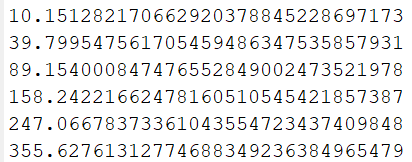
\includegraphics[scale = 0.7]{firstEigenValues.png}
    \end{center}
    See attached code for additional details.
\end{itemize}

\section*{Exercise 3.}
Consider the following diffusion-advection equation
\[u_t(x,t) + au_x(x,t) = \epsilon u_{xx}(x,t), \;\; x \in [0, \pi]\]
with periodic boundary condition
\[u(0,t) = u(\pi,t)\]
and initial condition
\[u(x,0) = \eta(x)\]
\begin{itemize}
    \item[(a)] Discretize the above PDE by a forward Euler scheme in time (with a centered difference scheme in space) on a uniform mesh $(x_j, t_n) = (jh,nk)$, $0 \leq j \leq m + 1$ ; $0 \leq n \leq N$, where $h$ and $k$ are step sizes.
    \newline\newline
    Using centered differences for $u$ in space, we have the following schemes for the first and second spatial derivatives, respectively:
    \begin{align*}
        u_x &\approx \frac{U^n_{j+1} - U^n_{j-1}}{2h^2} \\
        u_{xx} &\approx \frac{U^n_{j+1} - 2U_j^n + U^n_{j-1}}{h^2} \\
    \end{align*}
    and the forward Euler scheme for space takes the following form:
    \[u_t \approx \frac{U^{n+1}_j - U^n_j}{k}\]
    Putting this together, we find the following discretization scheme for the diffusion-advection equation:
    \[\frac{U_j^{n+1} - U_j^n}{k} + a\frac{U_{j+1}^n - U_{j-1}^n}{2h^2} = \epsilon\frac{U_{j-1}^n - 2U_j^n + U^n_{j+1}}{h^2}\]
    Solving the scheme for $U_j^{n+1}$, we find the following:
    \[U_j^{n+1} = U_j^n + \frac{k}{h^2}\left[-\frac{a}{2}(U_{j+1}^n - U_{j-1}^n) + \epsilon(U_{j-1}^n - 2U_j^n + U_{j+1}^n)\right]\]

    \item[(b)] Use von Neumann stability analysis to determine the amplification factor $g(\xi)$ of this scheme. What is the largest time step $\Delta t (= k)$ that makes this scheme stable, for a given $a, \epsilon$?
    \newline\newline
    Recall that von Neumann stability analysis involves replacing 
    \[U^n_j = [g(\xi)]^ne^{i\xi jh}\]
    applying this to our scheme, we find the following:
    \[g(\xi)^{n+1}e^{i\xi jh} = g(\xi)^ne^{i\xi jh} + \nu[-a(g(\xi)^ne^{i\xi(j+1)h} - g(\xi)^ne^{i\xi(j-1)h}) + 2\epsilon(g(\xi)^ne^{i\xi(j-1)h}-2g(\xi)^ne^{i\xi jh}+g(\xi)^ne^{i\xi(j-1)h})]\]
    where $\nu = k/(2h^2)$.
    \newline
    Dividing each side by $g(\xi)^ne^{i\xi jh}$, we have
    \[g(\xi) = 1 + \nu[-a(e^{i\xi h} - e^{-i\xi h}) + 2\epsilon(e^{-i\xi h} - 2 + e^{i\xi h})]\]
    which becomes
    \begin{align*}
        g(\xi) &= 1 + \nu[-2ia\sin{(\xi h)} + 2\epsilon(2\cos{(\xi h)} - 2)] \\
        &= 1 - \nu[8\sin^2{(\xi h/2)} + 2ia\sin{(\xi h)}] \\
    \end{align*}
    and since von Neumann analysis requires $|g(\xi)| \leq 1$, we have
    \begin{align*}
        &|g(\xi)|^2 = [1 - 8\epsilon\nu\sin^2(\xi h/2)]^2 + 4a^2\nu^2\sin^2(\xi h) \leq 1 \\
        &1 - 16\epsilon\nu\sin^2(\xi h/2) + 64\epsilon^2\nu^2\sin^4(\xi h/2) + 4a^2\nu^2\sin^2(\xi h) \leq 1 - 8\epsilon\nu\sin^2(\xi h/2)+ 16\epsilon^2\nu^2 + 4a^2\nu^2 \leq 1 \\
        &\nu^2(4a^2 + 64\epsilon^2) \leq 16\epsilon\nu \\
        &\nu \leq \frac{4 \epsilon}{a^2 + 16\epsilon^2} \\
    \end{align*}
    Then the largest time step that makes this method stable is given by
    \[k = \frac{8\epsilon h^2}{a^2 + 16\epsilon^2}\]
\end{itemize}


\section*{Exercise 4.}
Consider the so-called $\theta$-method for ODEs $u'(t) = f(u(t),t)$:
\[U^{n+1} = U^n + k[(1-\theta)f(U^n,t_n) + \theta f(U^{n+1}, t_{n+1})],\]
where $\theta$ is a fixed parameter. Note that $\theta = 0, 1/2, 1$ all give familiar methods.
\begin{itemize}
    \item[(1)] Show that this method is A-stable for $\theta \geq 1/2$
    \newline\newline
    Making the substitution $f(u(t),t) = \lambda u(t)$, our method takes the form
    \begin{align*}
        U^{n+1} &= U^n + k((1-\theta)\lambda U^n + \theta \lambda U^{n+1}) \\
        &= U^n + k(1-\theta)\lambda U^n + k\theta\lambda U^{n+1} \\
        U^{n+1}(1 - k\lambda\theta) &= (1+k(1-\theta)\lambda)U^n \\ 
        U^{n+1} &= \frac{1 + k\lambda(1 - \theta)}{1 - k\lambda\theta}U^n \\
    \end{align*}
    Let $z = k\lambda$. Then the above becomes
    \begin{align*}
        U^{n+1} &= \frac{1 + (1-\theta)z}{1 - \theta z}U^n \\
        &= R(z)U^n \\
    \end{align*}
    where $R(z) = \frac{1 + (1-\theta)z}{1 - \theta z}$. To analyze the stability region, we must find $\theta$ such that $|R(z)| \leq 1$. Well,
    \begin{align*}
        |R(z)| &= \left| \frac{1 + (1 - \theta)z}{1 - \theta z}\right| \leq 1\\
        |1 + (1 - \theta)z| &\leq |1 - \theta z| \\
    \end{align*}
    let $z = x + iy$ where $x,y \in \mathbb{R}$. Then we have
    \begin{align*}
        |1 + (1 - \theta)(x + iy)| &\leq |1 - \theta(x + iy)| \\
        (1 + (1-\theta)x)^2 + y^2(1-\theta)^2 &\leq (1-\theta x)^2 + (\theta y)^2 \\
        1 + 2(1-\theta)x + (1 - 2\theta + \theta^2)x^2 + y^2(1 - 2\theta + \theta^2) &\leq 1 - 2\theta x + \theta^2x^2 + \theta^2y^2 \\
        y^2(1-2\theta) \leq -(1-2\theta)x^2 - 2x \\
    \end{align*}
    Notice for $\theta = 1/2$, we get $x \leq 0$ for the above inequality, which is precisely the definition of A-stability. Now, let us inspect the case where $\theta \neq 1/2$. Notice, if we complete the square in $x$ and $y$ in the above inequalities, we find the following:
    \[\left(x + \frac{1}{1 - 2\theta}\right)^2 + y^2 \leq \left(\frac{1}{1 - 2\theta}\right)^2\]
    Notice that the above inequality corresponds to a filled in circle centered at $(1/(1-2\theta), 0)$ for $0 \leq \theta < 1/2$. For $\theta > 1/2$, we have $1 - 2\theta < 0$, so we may rewrite the equation of the circle above by
    \[\left(x - \frac{1}{2\theta-1} \right)^2 + y^2 \geq \left(\frac{1}{2\theta - 1}\right)^2\]
    which corresponds to the plane filled in with the circle of radius $1/(2\theta - 1)$ centered at $(1/(2\theta - 1), 0)$ cut out. Thus, for $\theta > 1/2$, we have this method is A-stable.
    \newline
    Finally, for $\theta \geq 1/2$, this method is A-stable.

    \item[(2)] Plot the stability region $\mathcal{S}$ for $\theta = 0, 1/4, 1/2, 3/4, 1$ and comment on how the stability region will look for other values of $\theta$.
    \newline\newline
    Implementing the above inequalities into MATLAB, we find for $\theta = 0, 1/4, 1/2, 3/4, 1$:
    \begin{center}
        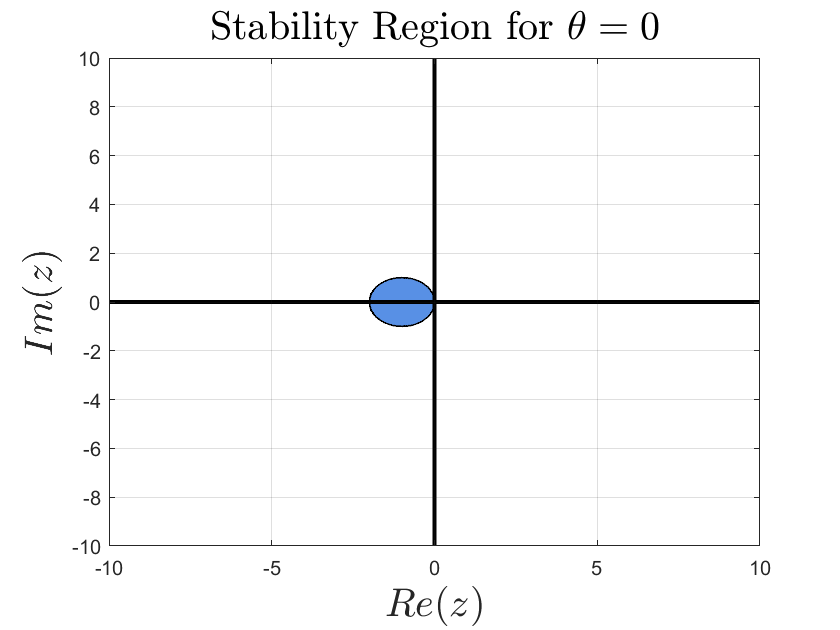
\includegraphics[scale = 0.25]{stabilityregion0.png}
        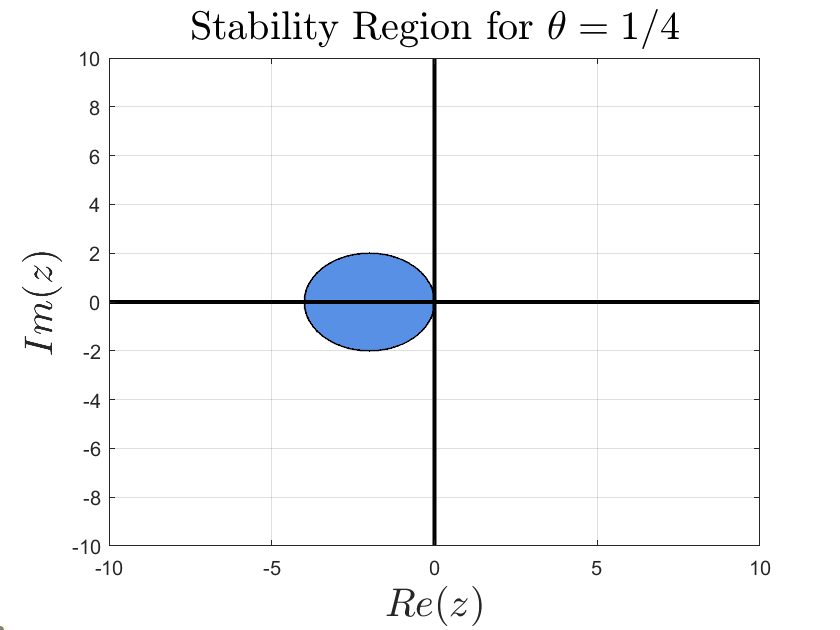
\includegraphics[scale = 0.25]{stabilityregion0.25.png}
        \newline
        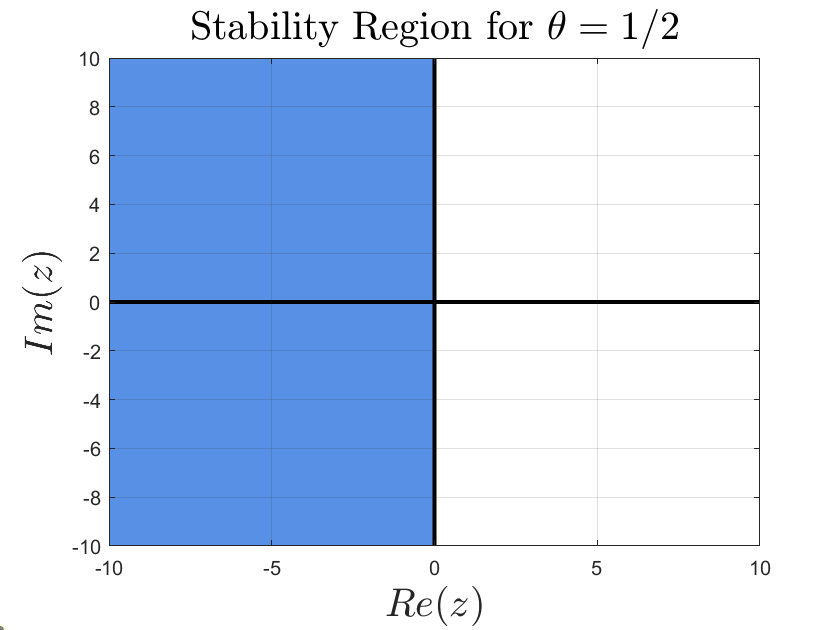
\includegraphics[scale = 0.25]{stabilityregion0.5.png}
        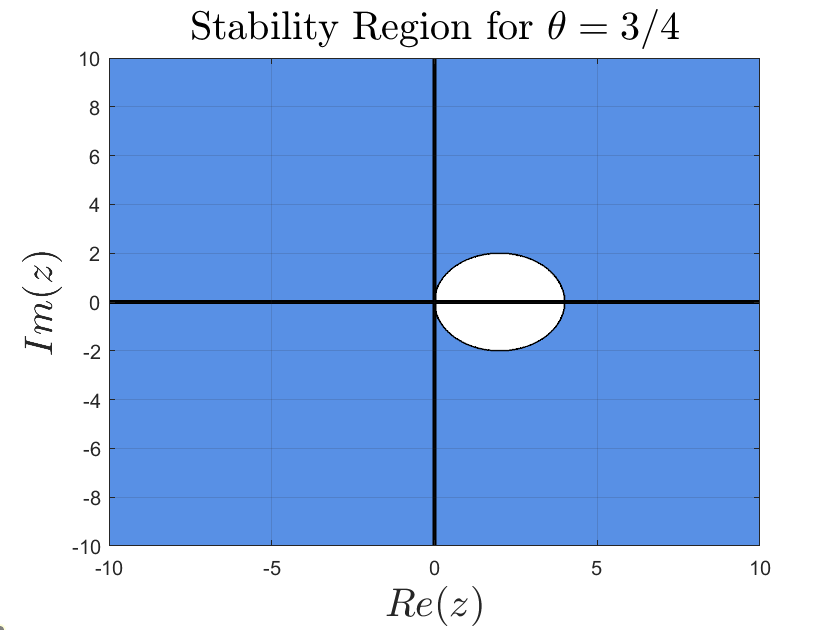
\includegraphics[scale = 0.25]{stabilityregion0.75.png}
        \newline
        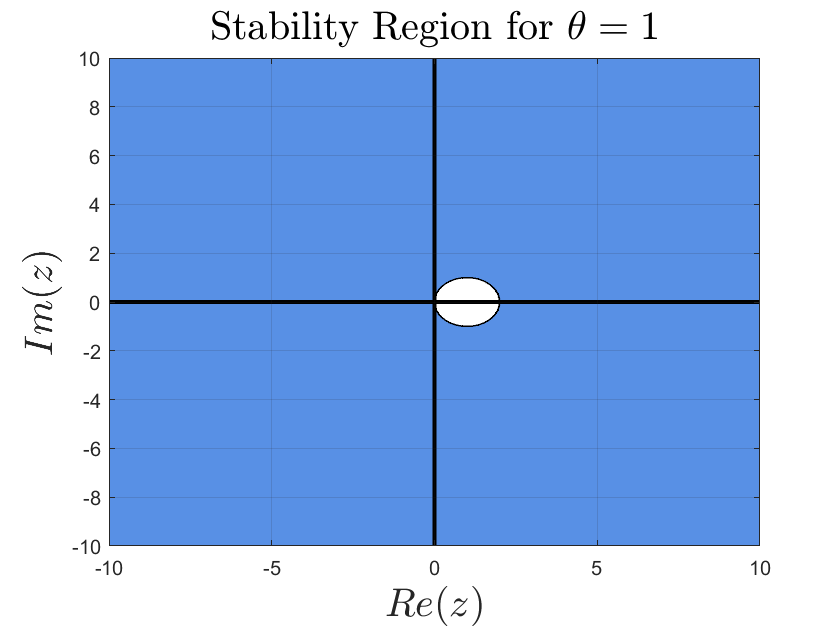
\includegraphics[scale = 0.25]{stabilityregion1.png}
    \end{center}
    See attached code for additional details. For other values of theta, whenever $0 < \theta < 1/2$, we have a filled in circle on the left half of the complex plane, whereas when $1/2 < \theta < 1$, we have the entire plane with a circle cut out on the right half of the complex plane.
    
\end{itemize}

\section*{Exercise 5.}
The PDE $u_t = \kappa u_{xx} - \gamma u$ models a diffusion with decay provided $\kappa > 0$ and $\gamma > 0$.
\newline\newline
Consider methods of the form
\[U_j^{n+1} = U^n_j + \kappa \frac{k}{2h^2}[U^n_{j-1} - 2U^n_j + U_{j+1}^n + U^{n+1}_{j-1} - 2U_j^{n+1} + U_{j+1}^{n+1}] - \kappa \gamma[(1-\theta)U^n_j + \theta U_j^{n+1}]\]
where $\theta$ is a parameter. 
In particular, if $\theta = 1/2$ then the decay term is modeled with the same centered-in-time approach as the diffusion term and the method can be obtained by applying the Trapezoidal method to the MOL formulation of the PDE. 
If $\theta = 0$ then the decay term is handled explicitly. 
For more general reaction-diffusion equations it may be advantageous to handle the reaction terms explicitly since these terms are generally nonlinear, so making them implicit would require solving nonlinear systems in each time step (whereas handling the diffusion term implicitly only gives a linear system to solve in each time step).
\begin{itemize}
    \item[(1)] By computing the local truncation error, show that this method is $\mathcal{O}(k^p + h^2)$ accurate, where $p = 2$ if $\theta = 1/2$ and $p = 1$ otherwise.
    \newline\newline
    To begin, let us Taylor expand $u_{j-1}^n$, $u_{j+1}^n$, and $u_j^{n+1}$:
    \begin{align*}
        u_{j-1}^n &= u_j^n - h\partial_xu_j^n + \frac{h^2}{2}\partial_x^2u_j^n - \frac{h^3}{3!}\partial_x^3u_j^n + \frac{h^4}{4!}\partial_x^4 + \mathcal{O}(h^5) \\
        u_{j+1}^n &= u_j^n + h\partial_xu_j^n + \frac{h^2}{2}\partial_x^2u_j^n + \frac{h^3}{3!}\partial_x^3u_j^n + \frac{h^4}{4!}\partial_x^4 + \mathcal{O}(h^5) \\
        u_j^{n+1} &= u_j^n + k\partial_tu_j^n + \frac{k^2}{2}\partial_t^2u_j^n + \frac{k^3}{3!}\partial_t^3u_j^n + \frac{k^4}{4!}\partial_t^4 + \mathcal{O}(k^5) \\
    \end{align*}
    Then we can see
    \begin{align*}
        (u_{j-1}^n - 2u_j^n + u_{j+1}^n) &= \frac{1}{2}\partial_x^2u_j^n + \frac{h^2}{4!}\partial_x^4u_j^n + \mathcal{O}(h^3) \\
    \end{align*}
    Now let's expand the $u_{j-1}^{n+1}$ and $u_{j+1}^{n+1}$ terms:
    \begin{align*}
        u_{j-1}^{n+1} &= u_j^n - h\partial_xu_j^n + k\partial_tu_j^n + \frac{h^2}{2}\partial_x^2u_j^n + \frac{k^2}{2}\partial_t^2u_j^n - hk\partial_{xt}u_j^n - \frac{h^3}{3!}\partial_x^3u_j^n + \frac{k^3}{3!}\partial_t^3u_j^n \cdots \\
        &\cdots - \frac{hk^2}{2}\partial_{xtt}u_j^n + \frac{h^2k}{2}\partial_{xxt}u_j^n + \frac{h^4}{4!}\partial_x^4u_j^n + \frac{k^4}{4!}\partial_t^4u_j^n + \frac{h^2k^2}{4}\partial_{xxtt}u_j^n \cdots \\
        &\cdots - \frac{h^3k}{3!}\partial_{xxxt}u_j^n - \frac{hk^3}{3!}\partial_{xttt}u_j^n + \mathcal{O}(h^5 + k^5) \\
        u_{j+1}^{n+1} &= u_j^n + h\partial_xu_j^n + k\partial_tu_j^n + \frac{h^2}{2}\partial_x^2u_j^n + \frac{k^2}{2}\partial_t^2u_j^n + hk\partial_{xt}u_j^n + \frac{h^3}{3!}\partial_x^3u_j^n + \frac{k^3}{3!}\partial_t^3u_j^n \cdots \\
        &\cdots + \frac{hk^2}{2}\partial_{xtt}u_j^n + \frac{h^2k}{2}\partial_{xxt}u_j^n + \frac{h^4}{4!}\partial_x^4u_j^n + \frac{k^4}{4!}\partial_t^4u_j^n + \frac{h^2k^2}{4}\partial_{xxtt}u_j^n \cdots \\
        &\cdots + \frac{h^3k}{3!}\partial_{xxxt}u_j^n + \frac{hk^3}{3!}\partial_{xttt}u_j^n + \mathcal{O}(h^5 + k^5) \\
    \end{align*}
    Then we have
    \begin{align*}
        \frac{1}{2h^2}(u_{j+1}^{n+1} + u_{j-1}^{n+1} - 2u_J^{n+1}) &= \frac{1}{2}\partial_x^2u_j^n + \frac{k}{2}\partial_{xxt}u_j^n + \frac{h^2}{4!}\partial_x^4u_j^n + \frac{k^2}{4}u_j^n + \mathcal{O}(h^3 + k^5) \\
    \end{align*}
    Putting it together, for the first part of the method, we have
    \begin{align*}
        &\kappa\frac{1}{2h^2}[u_{j-1}^n + u_{j+1}^n - 2u_j^n + u_{j+1}^{n+1} + u_{j-1}^{n+1} - 2u_j^{n+1}] = \\
        &= \partial_x^2u_j^n + \frac{h^2}{12}\partial_x^4u_j^n + \frac{k}{2}\partial_{xxt}u_j^n + \frac{k^2}{4}\partial_{xxtt}u_j^n + \mathcal{O}(h^3 + k^5) \\
    \end{align*}
    Additionally, for the left hand side, we have
    \begin{align*}
        \frac{u_j^{n+1} - u_j^n}{k} &= \partial_tu_j^n + \frac{k}{2}\partial_t^2u_j^n + \frac{k^2}{3!}\partial_t^3u_j^n + \mathcal{O}(k^3) \\
    \end{align*}
    Now, for the "$\theta$ part" of the method,
    \begin{align*}
        \theta u_j^{n+1} &= \theta\left[u_j^n + k\partial_tu_j^n + \frac{k^2}{2}\partial_t^2u_j^n + \frac{k^3}{3!}\partial_t^3u_j^n + \mathcal{O}(k^4)\right] \\
    \end{align*}
    so
    \begin{align*}
        (1-\theta)u_j^n + \theta u_j^{n+1} &= u_j^n + \theta k\partial_tu_j^n + \theta\frac{k^2}{2}\partial_t^2u_j^n + \theta\frac{k^3}{3!}\partial_t^3u_j^n + \mathcal{O}(k^4) \\
    \end{align*}
    Putting all these pieces together, we find the following for the local truncation error:
    \begin{align*}
        \tau_n = \partial_tu_j^n + \frac{k}{2}\partial_t^2u_j^n + \frac{k^2}{3!}\partial_t^3u_j^n - &\kappa\left(\partial_x^2u_j^n + \frac{h^2}{12}\partial_x^4u_j^n + \frac{k}{2}\partial_{xxt}u_j^n + \frac{k^2}{4}\partial_{xxtt}u_j^n\right) \cdots \\
        &\cdots + \gamma\left(u_j^n + \theta k\partial_tu_j^n + \theta\frac{k^2}{2}\partial_t^2u_j^n + \theta\frac{k^3}{3!}\partial_t^3u_j^n\right) \\
    \end{align*}
    Notice that for $\theta = 1/2$, using our differential equation, $u_t = \kappa u_{xx} - \gamma u$, and differentiating with respect to $t$ to get the relation $u_{tt} = \kappa u_{xxt} - \gamma u_t$, the above expression for the truncation error reduces to
    \begin{align*}
        \tau_n &= \frac{k^2}{3!}\partial_t^3u_j^n - \kappa\left[\frac{h^2}{12}\partial_x^4u_j^n + \frac{k^2}{4}\partial_{xxtt}u_j^n\right] + \gamma\left[\frac{k^2}{4}\partial_t^2u_j^n + \frac{k^3}{12}\partial_t^3u_j^n\right] \\
        &= \mathcal{O}(k^2 + h^2) \\
    \end{align*}
    and if $\theta \neq 1/2$, it is clear to see that the method will be $\mathcal{O}(k + h^2)$.

    \item[(2)] Using von Neumann analysis, show that this method is unconditionally stable if $\theta \geq 1/2$.
    \newline\newline
    Replacing $U_j^n = [g(\xi)]^ne^{i\xi jh}$, the discretization scheme becomes
    \begin{align*}
        [g(\xi)]^{n+1}e^{i\xi jh} &= [g(\xi)]^ne^{i\xi j h} + \kappa\frac{k}{2h^2}([g(\xi)]^ne^{i\xi(j-1)h} - 2[g(\xi)]^ne^{i\xi jh} + [g(\xi)]^ne^{i\xi(j+1)h} \cdots \\
        &\cdots + [g(\xi)]^{n+1}e^{i\xi(j+1)h} -2[g(\xi)]^{n+1}e^{i\xi j h} + [g(\xi)]^{n+1}e^{i\xi(j+1)h}) \cdots \\
        & - k\gamma\left[(1-\theta)[g(\xi)]^ne^{i\xi jh} + \theta[g(\xi)]^{n+1}e^{i\xi jh}\right] \\
    \end{align*}
    Cancelling out common factors, we have
    \begin{align*}
        g(\xi) &= 1 + \kappa\frac{k}{2h^2}\left[e^{-i\xi h} - 2 + e^{i\xi h} + g(\xi)e^{-i\xi h} - 2g(\xi) + g(\xi)e^{i\xi h}\right] - k\gamma[(1-\theta) + \theta g(\xi)] \\
    \end{align*}
    which becomes
    \begin{align*}
        g(\xi) &= 1 + \kappa\frac{k}{2h^2}\left[-4\sin^2\left(\frac{\xi h}{2}\right) - 4g(\xi)\sin^2\left(\frac{\xi h}{2}\right)\right] - k\gamma[(1-\theta) + \theta g(\xi)]
    \end{align*}
    collecting common terms and solving for $g(\xi)$, we find
    \begin{equation}
        g(\xi) = \frac{1 - 4\kappa\frac{k}{2h^2}\sin^2\left(\frac{\xi h}{2}\right) - k\gamma(1 - \theta)}{1 + 4\kappa\frac{k}{2h^2}\sin^2\left(\frac{\xi h}{2}\right) + k\gamma \theta}
    \end{equation}
    Notice for $\theta = 1/2$, $g(\xi)$ becomes
    \[g(\xi) = \frac{1 - 4\kappa\frac{k}{2h^2}\sin^2\left(\frac{\xi h}{2}\right) - \frac{1}{2}k\gamma}{1 + 4\kappa\frac{k}{2h^2}\sin^2\left(\frac{\xi h}{2}\right) + \frac{1}{2}k\gamma}\]
    Since $\kappa, \gamma > 0$, we can see that the numerator will be lower in magnitude than the denominator, so $|g(\xi)| \leq 1$ will be satisfied. Similarly, for $ 1/2 < \theta \leq 1$, the same logic holds, so $|g(\xi)| \leq 1$ will also be satisfied, regardless of $h$ and $k$. Thus, for $\theta \geq 1/2$, the method is unconditionally stable.
    
    \item[(3)] Show that if $\theta = 0$ then the method is stable provided $k \leq 2/\gamma$, independent of $h$.
    \newline\newline
    Using equation (1) in part (2), taking the derivative to find the maximum value of $g(\xi)$, we find 
    \begin{align*}
        2 + 2k\gamma\theta = k\gamma\\
    \end{align*}
    Then for $\theta = 0$, we have
    \[k = \frac{2}{\gamma}\]
    Since this is the maximum value of $k$, we have in generality,
    \[k \leq \frac{2}{\gamma}\]
    
\end{itemize}

\end{document}
